\section{RINA on WiFi}

Following the introduction to the RINA alternative in section~\ref{sec:RINAalternative} we will now take a closer look to RINA over WiFi on Android. What the exact needs are for this implementation and where special focus will be needed. We kick this section off with a piece about IEEE 802.11 MAC protocol. Followed by the WiFi Shim-DIF. Finally we will take a closer look at the Android restrictions (compared to Linux).

\subsection{IEEE 802.11 Media Access Control}

In this subsection we will address the WiFi MAC\footnote{802.11 Media Access Control} \citep{matthewgast2005}. Since the protocol covers both layer 1 (physical layer) and a part of layer 2 (Media Access Control) we will limit ourselves here to the layer 2 interaction. The IRATI project code will have to fit seamless on this protocol to ensure maximal optimization for wireless communication. In this light we must instantly make an important remark. In normal operation mode the device drivers for user devices will be set to \emph{STA} mode (Station infrastructure mode). This enables basic device functions, however two devices in STA mode will not be able to communicate with each other unless an Access Point (AP) is presented to communicate with. As can been seen in figure~\ref{fig:80211inframode}.

\begin{figure}[H]
    \centering
    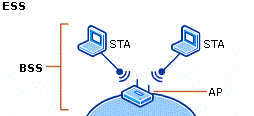
\includegraphics{figures/80211inframode}
    \caption{802.11 Infrastructure mode (STA and AP) \citep{website:80211microsoft}} 
    \label{fig:80211inframode}
\end{figure}

\npar

Drivers can also function in other modes, some of which will be handled later in this thesis, some who will not be handled at all. Other modes that drivers are capable of are \citep{website:80211wirelesskernel}: 
\begin{description}
	\item[AccessPoint (AP) infrastructure mode] Access Point for a master device in a network, normal mode for WiFi router. \emph{Not handled further}
	\item[Monitor (MON) mode] A passive mode that allows monitoring of all packets the device receives, can be double used in some devices. \emph{Used in testcases}
	\item[Ad-Hoc (IBSS) mode] Enables communication between other ad-hoc devices without AP (figure~\ref{fig:80211adhoc}). \emph{Used in testcases}

\begin{figure}[H]
    \centering
    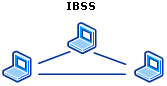
\includegraphics{figures/80211adhoc}
    \caption{802.11 Ad-hoc mode) \citep{website:80211microsoft}} 
    \label{fig:80211adhoc}
\end{figure}

	\item[Wireless Distribution System (WDS) mode] Enables communication between devices (mostly APs in a single ESS), uses the 4-addresses from the layer-2 header\footnote{Other modes only use these partially and mostly leave one or more fields empty}. \emph{Not handled further}
	\item[Mesh] Enables communication in Wireless Mesh Networks, used to set up intelligent, dynamic routes. \emph{Not handled further}
 \end{description}


\npar

For the initial part of this thesis we will leave the device in either STA or IBSS mode. This means that the drivers will \emph{translate} the 802.11 MAC-headers to 802.1q MAC-headers when in STA mode (see Appendix~\ref{chap:emailconvo}. If this happens in IBSS mode we will have to test or ask authorized sources\footnote{Linux Wireless Kernel group for example}. The difference can be seen in the figure below (figure~\ref{fig:80211vs8021q}). We see that the entire header (Ethernet) becomes quite a bit easier to understand in STA mode. Since the IRATI project already has a working Ethernet Shim-DIF this will, under normal conditions, fit on this MAC header in STA mode. When expanding further down the road we will have to implement a Shim-DIF capable of handling the 802.11 MAC header. 


\begin{figure}[H]
    \centering
    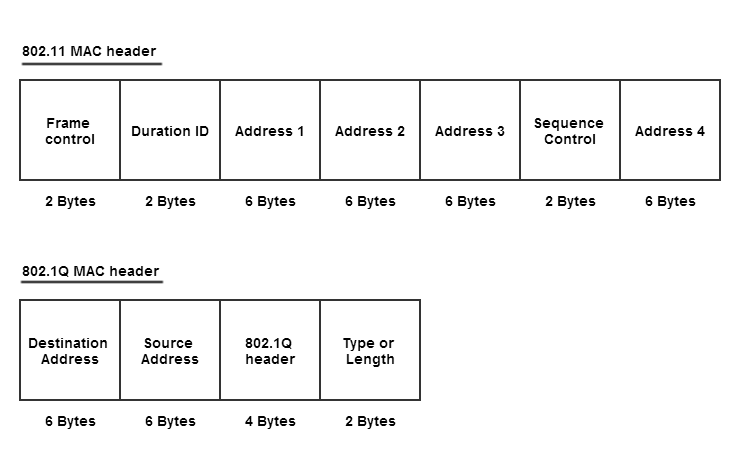
\includegraphics[width=0.8\textwidth]{figures/80211vs8021q}
    \caption{802.11 and 802.1q MAC headers} 
    \label{fig:80211vs8021q}
\end{figure}

\npar

Since WiFi (802.11) MAC headers have quite a lot more functions (30 bytes compared to 802.1q's 18 bytes) we will have to adjust the code for this. The functions that are added can potentially prove useful for the architecture and thus further study should be implemented. This research will focus on the overlap of functions between the MAC header and the functions provided by the IPC API. It can ultimately prove advantageous to use the full 802.11 header alongside with RINA instead of having drivers reform this header to a more easy to comprehend Ethernet MAC header. 


\subsection{Shim-DIF for wireless}

While under normal operation of the research question we delve further into the Shim-DIF over WiFi (see figure~\ref{fig:rinaoverwifi}. However, due to reasons stated in the previous segment we clearly see that this has now been reformed to:

\begin{figure}[H]
    \centering
    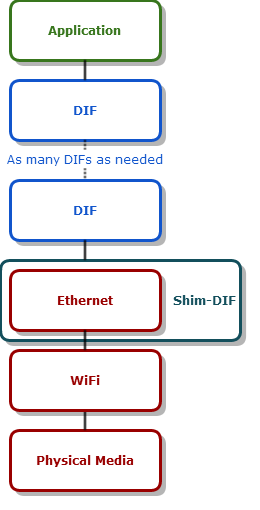
\includegraphics[width=0.4\textwidth]{figures/rinaoverwifi2}
    \caption{RINA over WiFi (updated)} 
    \label{fig:rinaoverwifi2}
\end{figure}

\npar
In normal conditions this means we can fully copy the code from IRATI we must remind ourselves that we are still working on another Operating System and this comes with consequences. These are handled in the next component. However if time allows this, we will take a closer look at the 802.11 packets and provide a Shim-DIF for the 802.11 standard (802.11n specifically). This provides a base for other developers who wish to update drivers further down to road to make said drivers compatible with RINA. 

\subsection{Android restrictions}

While Android is a UNIX-like operating system and based on Linux, it does come with some restrictions. In this subdivision we will be comparing Android OS to the Linux OS. The reason for this is that the IRATI project already has a working RINA implementation on Linux and this will be used for the further work of this thesis. Secondly because Android is based on Linux operating system and its kernel. At one point in history the two operating systems shared a common kernel and while this common component is planned, it is currently not the same kernel. 
\npar
Before we can further inspect the Android operating system, compared to Linux OS, we first need to identify the differences between the \emph{Android kernel} and \emph{Linux kernel}. For most of this information we will be using a talk by John Stultz, comparing Android to a stock Linux kernel \citep{presentation:android_linux_kernel,website:android_linux_kernel}. The amount of changes is not that large as it comprises of around 25 000 lines of changes, compared to the entire 15 millions lines of code for the full kernel. This places the changes around \textasciitilde0.2\% of the total code. Of course some of these changes can have large impacts on the actual kernel itself. These changes will be discussed here. Some of the items in the Android patches include:
\begin{itemize}
	\item Ashmem
	\item Binder
	\item Pmem
	\item Logger
	\item Early suspend
	\item Wakelocks
	\item Various small \emph{hacks} to facilitate a mobile OS
	\item \ldots
\end{itemize}
Because a Linux kernel is meant for desktop and server hardware (both very similar), Android aims to improve in the hardware department. This allows the use of more and varied hardware through its kernel. A second large point of interest for Android is the power management. While traditional systems are just plugged in with the cable and thus don't need to worry as much about power. The opposite is true for mobile, battery powered devices where power management is of utmost importance. Another change between the two kernels is the way error reporting is done and the attempt to increase security on the Android kernel. Finally the Android kernel aims to improve performance, especially for its intended users, mobile platforms.
\\
Some of these changes to the original kernel have been talked about quite a bit, such as the wakelocks. However we find that these changes will not impact the current implementation of the IRATI stack into Android. Further down the road additional optimization can be acquired between the Android kernel and the IRATI stack. Also RINA will have to be able to work with Paranoid Networking so that networking does not become blocked by this feature in Android kernels. For this part further research will be conducted. 
\npar
As shown above, the current version (and future versions) of the Android kernel will not pose any problems for the IRATI stack. However, an operating system does not only comprise of its kernel. This is an important part and the aspect where we see the biggest change between Linux and Android. When looking at a structured overview of an operating system (UNIX-like), we see that libraries play a big part in the undertaking of an operating system. Here we find the biggest change between Android and Linux. While Linux uses glibc \citep{website:glibc} and Android uses the Bionic library \citep{github:bionic,website:c_lib_bionic}. 
\npar
The restrictions from the Bionic library that affect the inclusion of the IRATI stack on Android are mostly limited to the \cpp language. The way Bionic handles \cpp is quite unique as it aims to alter the use of \cpp as a whole. This issue here is the following: IRATI stack is build on \cpp. For the most part \cpp is still supported by the library, but it does come with some restrictions. Before we inspect those restrictions we must first look at the reason why the glibc was not used in the first place. This can be declared very fast and accurate. Glibc is a \emph{slow} and \emph{huge} library. While this is not an issue for systems that run on Linux (desktops, servers, \ldots) it does form a problem for small-scale mobile platforms. Another issue with glibc is that it falls under GPL (GNU General Public License) and the smaller version, uClibC falls under LGPL (Lesser GNU General Public License). This implies that everything that uses these libraries also falls under these licenses, something Google was looking to avoid. Hence the option to use a new library, Bionic, which uses as BSD license and thus can shield its applications from the GPL and LGPL licenses. Finally we must note that glibc is quite large and meant for high frequency processors, where bionic is a lot smaller and works very fast, even without high speed processors\footnote{High frequency CPUs are becoming available for mobile platforms at this very moment}.
\npar
Because the \cpp restrictions of the Bionic library are of utmost importance to this IRATI project inclusion we will now take a closer look at these restrictions. The most profound and important restriction is the lack of support for \cpp exceptions. Google engineers deemed these exceptions bloated and largely impractical for use thus the support for this was entirely cut. When people still want to use exceptions they are advised to try another library, add a library that does support these or switch to Java programming language in the userspace. This is an important change as the current IRATI project does use \cpp exceptions and thus the code will need to be retailored to fit seamless on the Android platform. Another option is to try and implement changes on Android so that the current IRATI project can be ported over. Secondly, Bionic does not contain a \cpp Standard Template Library. This is for obvious reasons to try and keep Bionic as small as possible. When applications wish to use a \cpp STL they will have to include one with the application or acquire it beforehand. Other changes bionic made can be viewed at Pthreads. These are threads that are standardized and should be compatible cross-platform. Some changes bionic made to these threads include: cancellation, pthread\_once(), pthread\_atfork(). Here it is recommended that when these functions are used in the original code, to revise the code and work around these changes. The changes are in place again to reduce the bloated code in glibc and endorse optimized coding. The final changes that bionic implements are the lack of support for wide and locale characters and some user-account-related functions. 
\npar
Finally we see that the biggest restrictions on Android come from the use of the Bionic library. This library limits some uses of \cpp and requires a bypass from the original application. We note that the IRATI project is written partially in \cpp and uses exceptions. This will require a workaround on either the operating system side or on the IRATI project. How this will be handled is one of the major questions in this thesis. 